\textbf{NOTE: We have already demoed to the TA for this course and have proven that our implementation of the MapReduce on Hadoop is correct and in working order.}

\begin{figure}[!htbp] 
 \frame{ 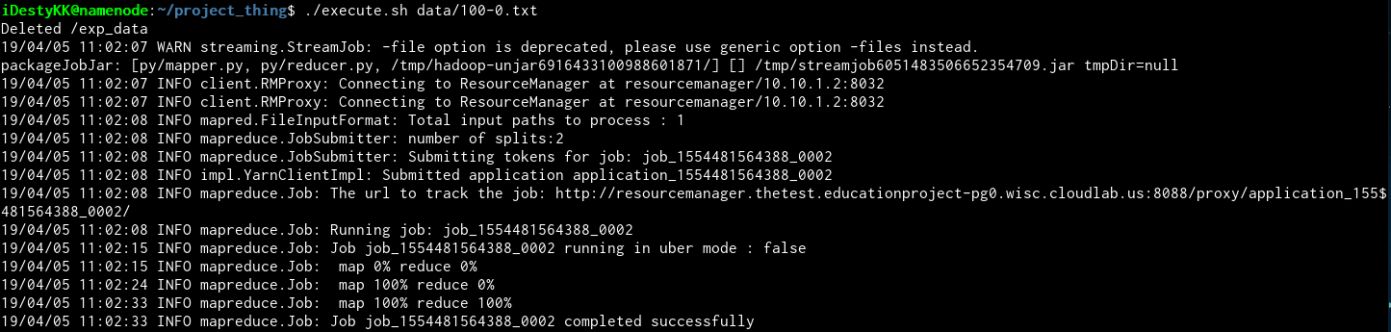
\includegraphics[width=\textwidth]{hadoop_1fileinput.png}}
  \caption{Proof of program running with one text input file}
\end{figure}

\begin{figure}[!htbp] 
 \frame{ 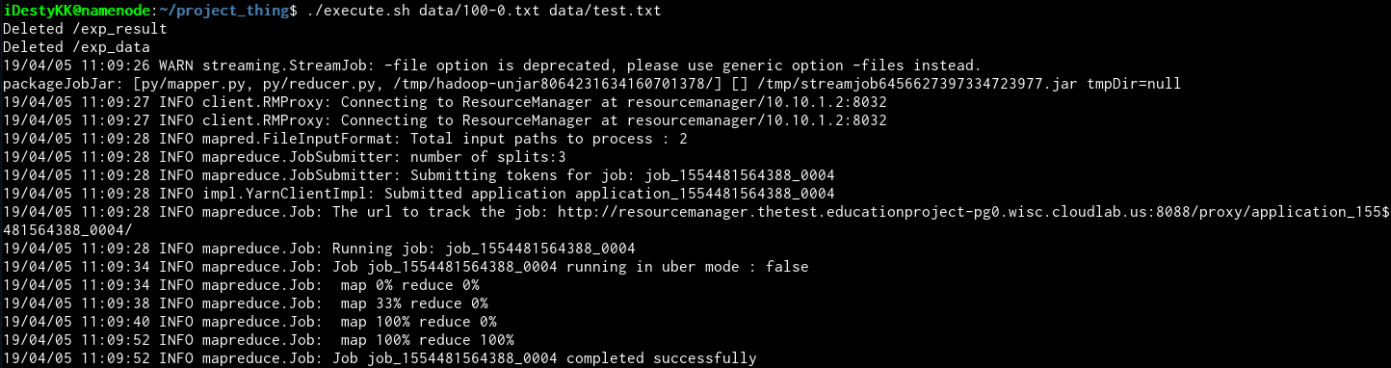
\includegraphics[width=\textwidth]{hadoop_2filesinput.png}}
  \caption{Proof of program running with multiple text input files}
\end{figure}

\begin{figure}[!htbp] 
 \frame{ 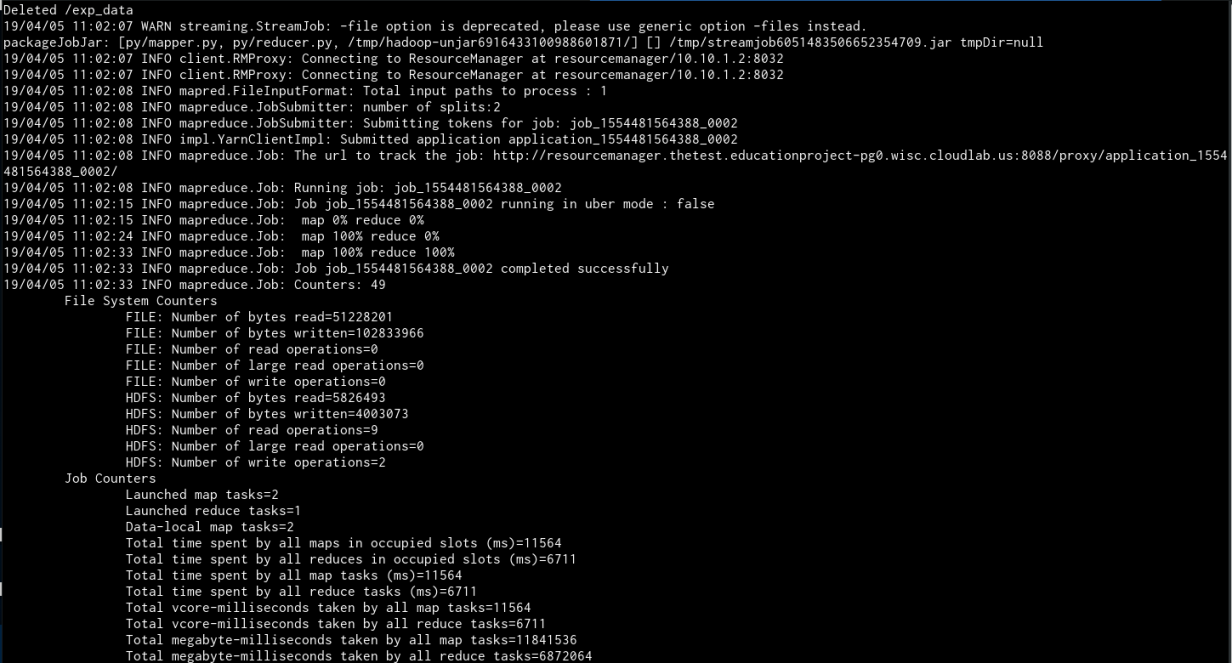
\includegraphics[width=\textwidth]{hadoop_codecomplete.png}}
  \caption{Proof of program completion}
\end{figure}

\begin{figure}[!htbp] 
 \frame{ 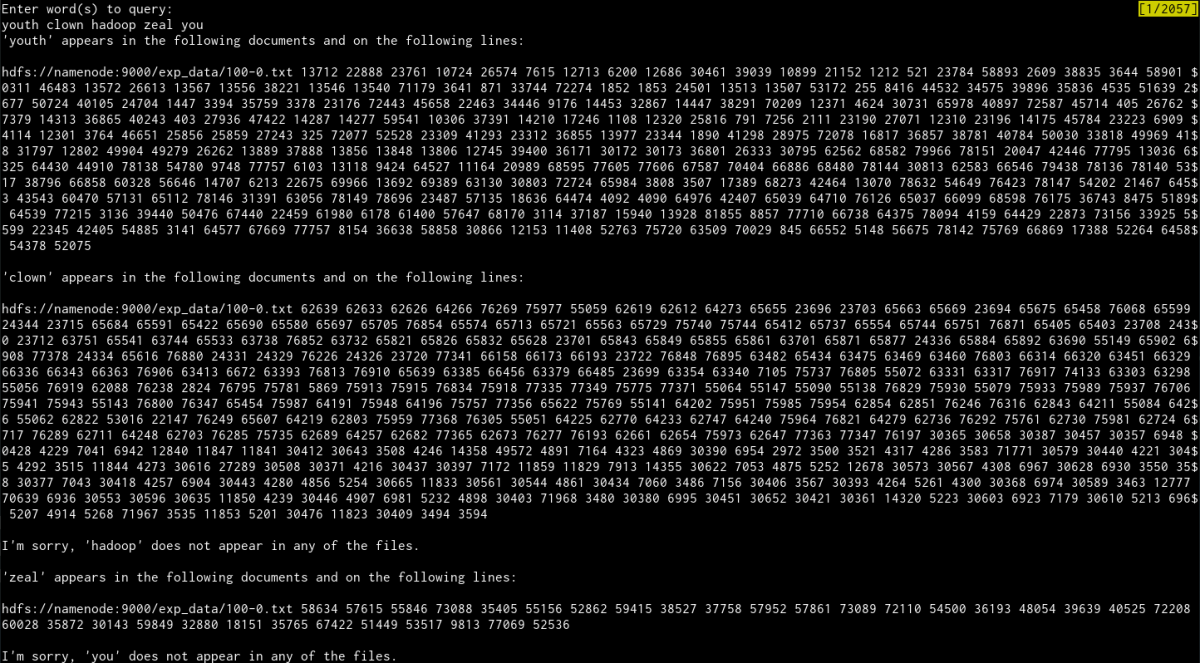
\includegraphics[width=\textwidth]{hadoop_query.png}}
  \caption{Query function showing line display for words in line, not in file, and the removal of stop words.}
\end{figure}